\begin{figure}[ht!]
  \centering
  \caption{Distribution of carbon intensities over expenditure quintiles} \label{fig:Quint}
  \begin{subfigure}[b]{\textwidth}
  \centering
    \caption{Distribution of carbon intensities over expenditure quintiles - Part A} \label{fig:Quint_A}
  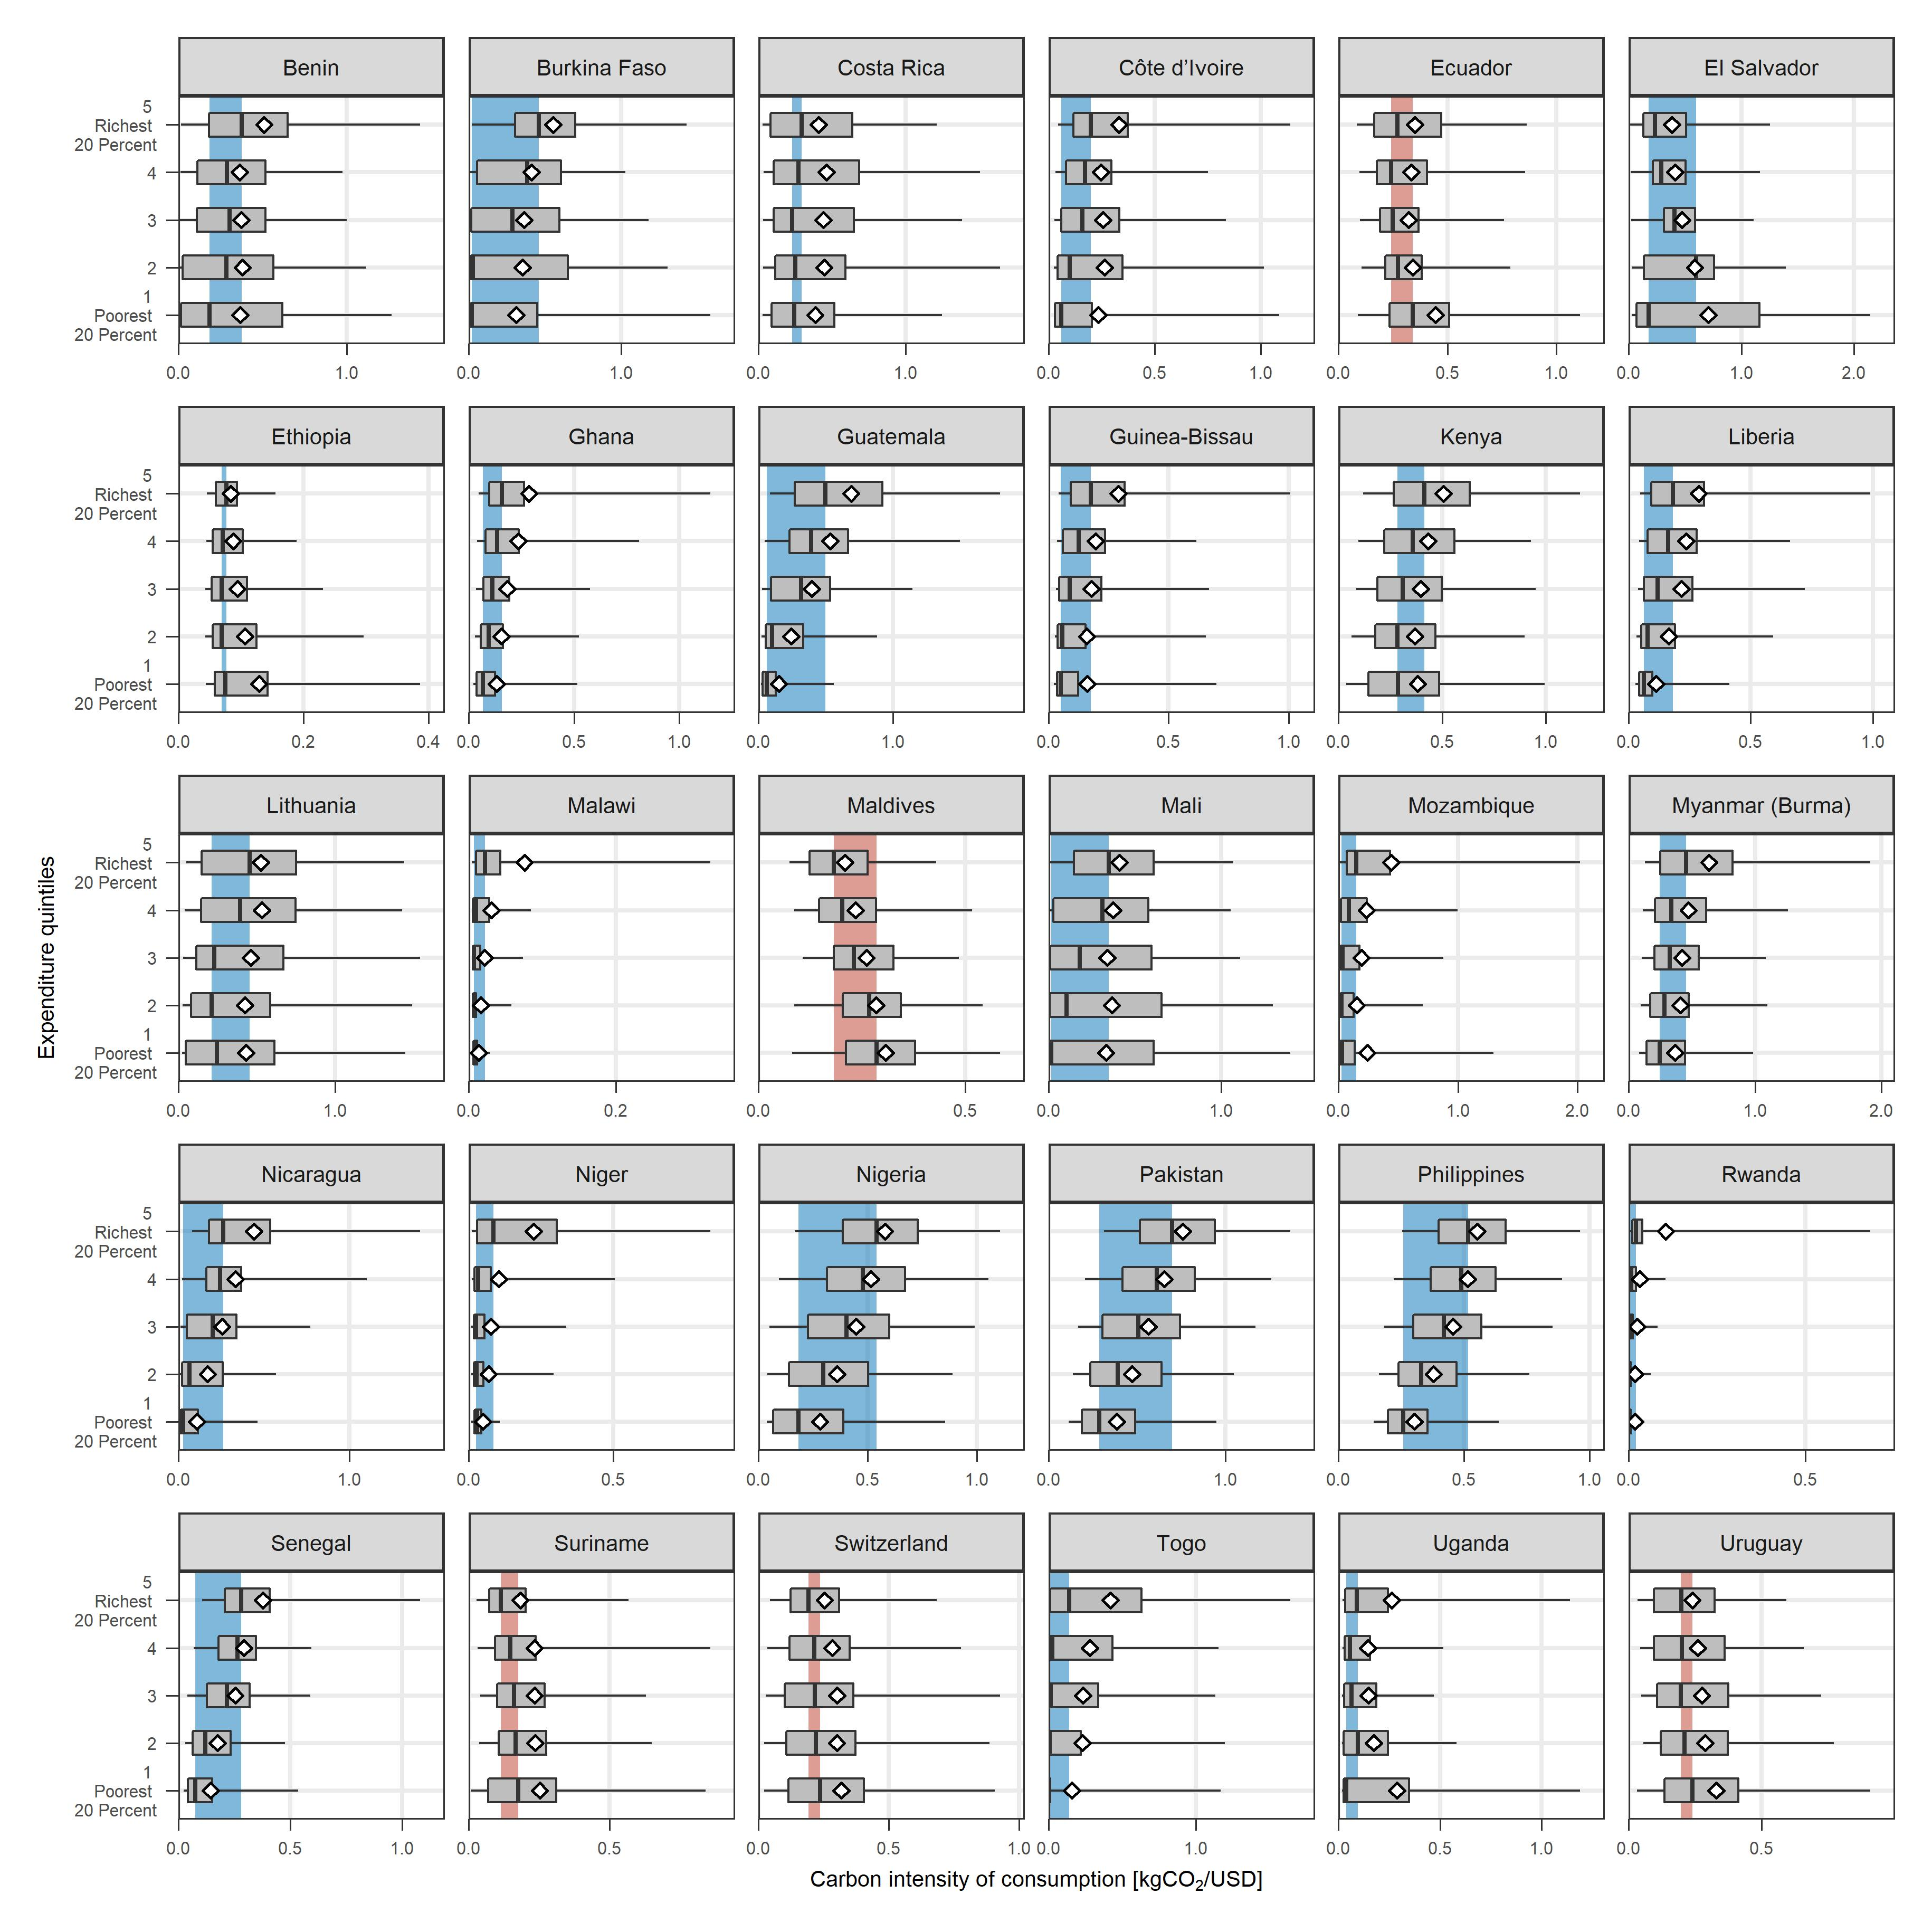
\includegraphics{1_Figures/Figures_Appendix/Figure_1_2017_Appendix_1.jpg}
  \begin{subcaption2}
    This figure displays the distribution of carbon intensity of consumption in kgCO$_{2}$/USD (x-axis) over expenditure quintiles (y-axis) for 30 countries. The first expenditure quintile comprises those 20\% of all households with least total expenditures per capita. The fifth expenditure quintile comprises those 20\% of all households with largest expenditures per capita. Within quintiles, boxes display the 25\textsuperscript{th} and the 75\textsuperscript{th} percentile; whiskers display the 5\textsuperscript{th} and 95\textsuperscript{th} percentile; rhombuses indicate the within-quintile average. Vertical coloured bands indicate the difference between the highest and the lowest quintile-level median carbon intensity of consumption. Blue bands indicate higher carbon intensities among richer households; red bands indicate higher carbon intensities among poorer households. See also Tables \ref{tab:A3} and \ref{tab:A7}.
  \end{subcaption2}
  \end{subfigure}
\end{figure}

\clearpage

\begin{figure}[ht!]\ContinuedFloat
   \begin{subfigure}[b]{\textwidth}
  \centering
      \caption{Distribution of carbon intensities over expenditure quintiles - Part B} \label{fig:Quint_B}
  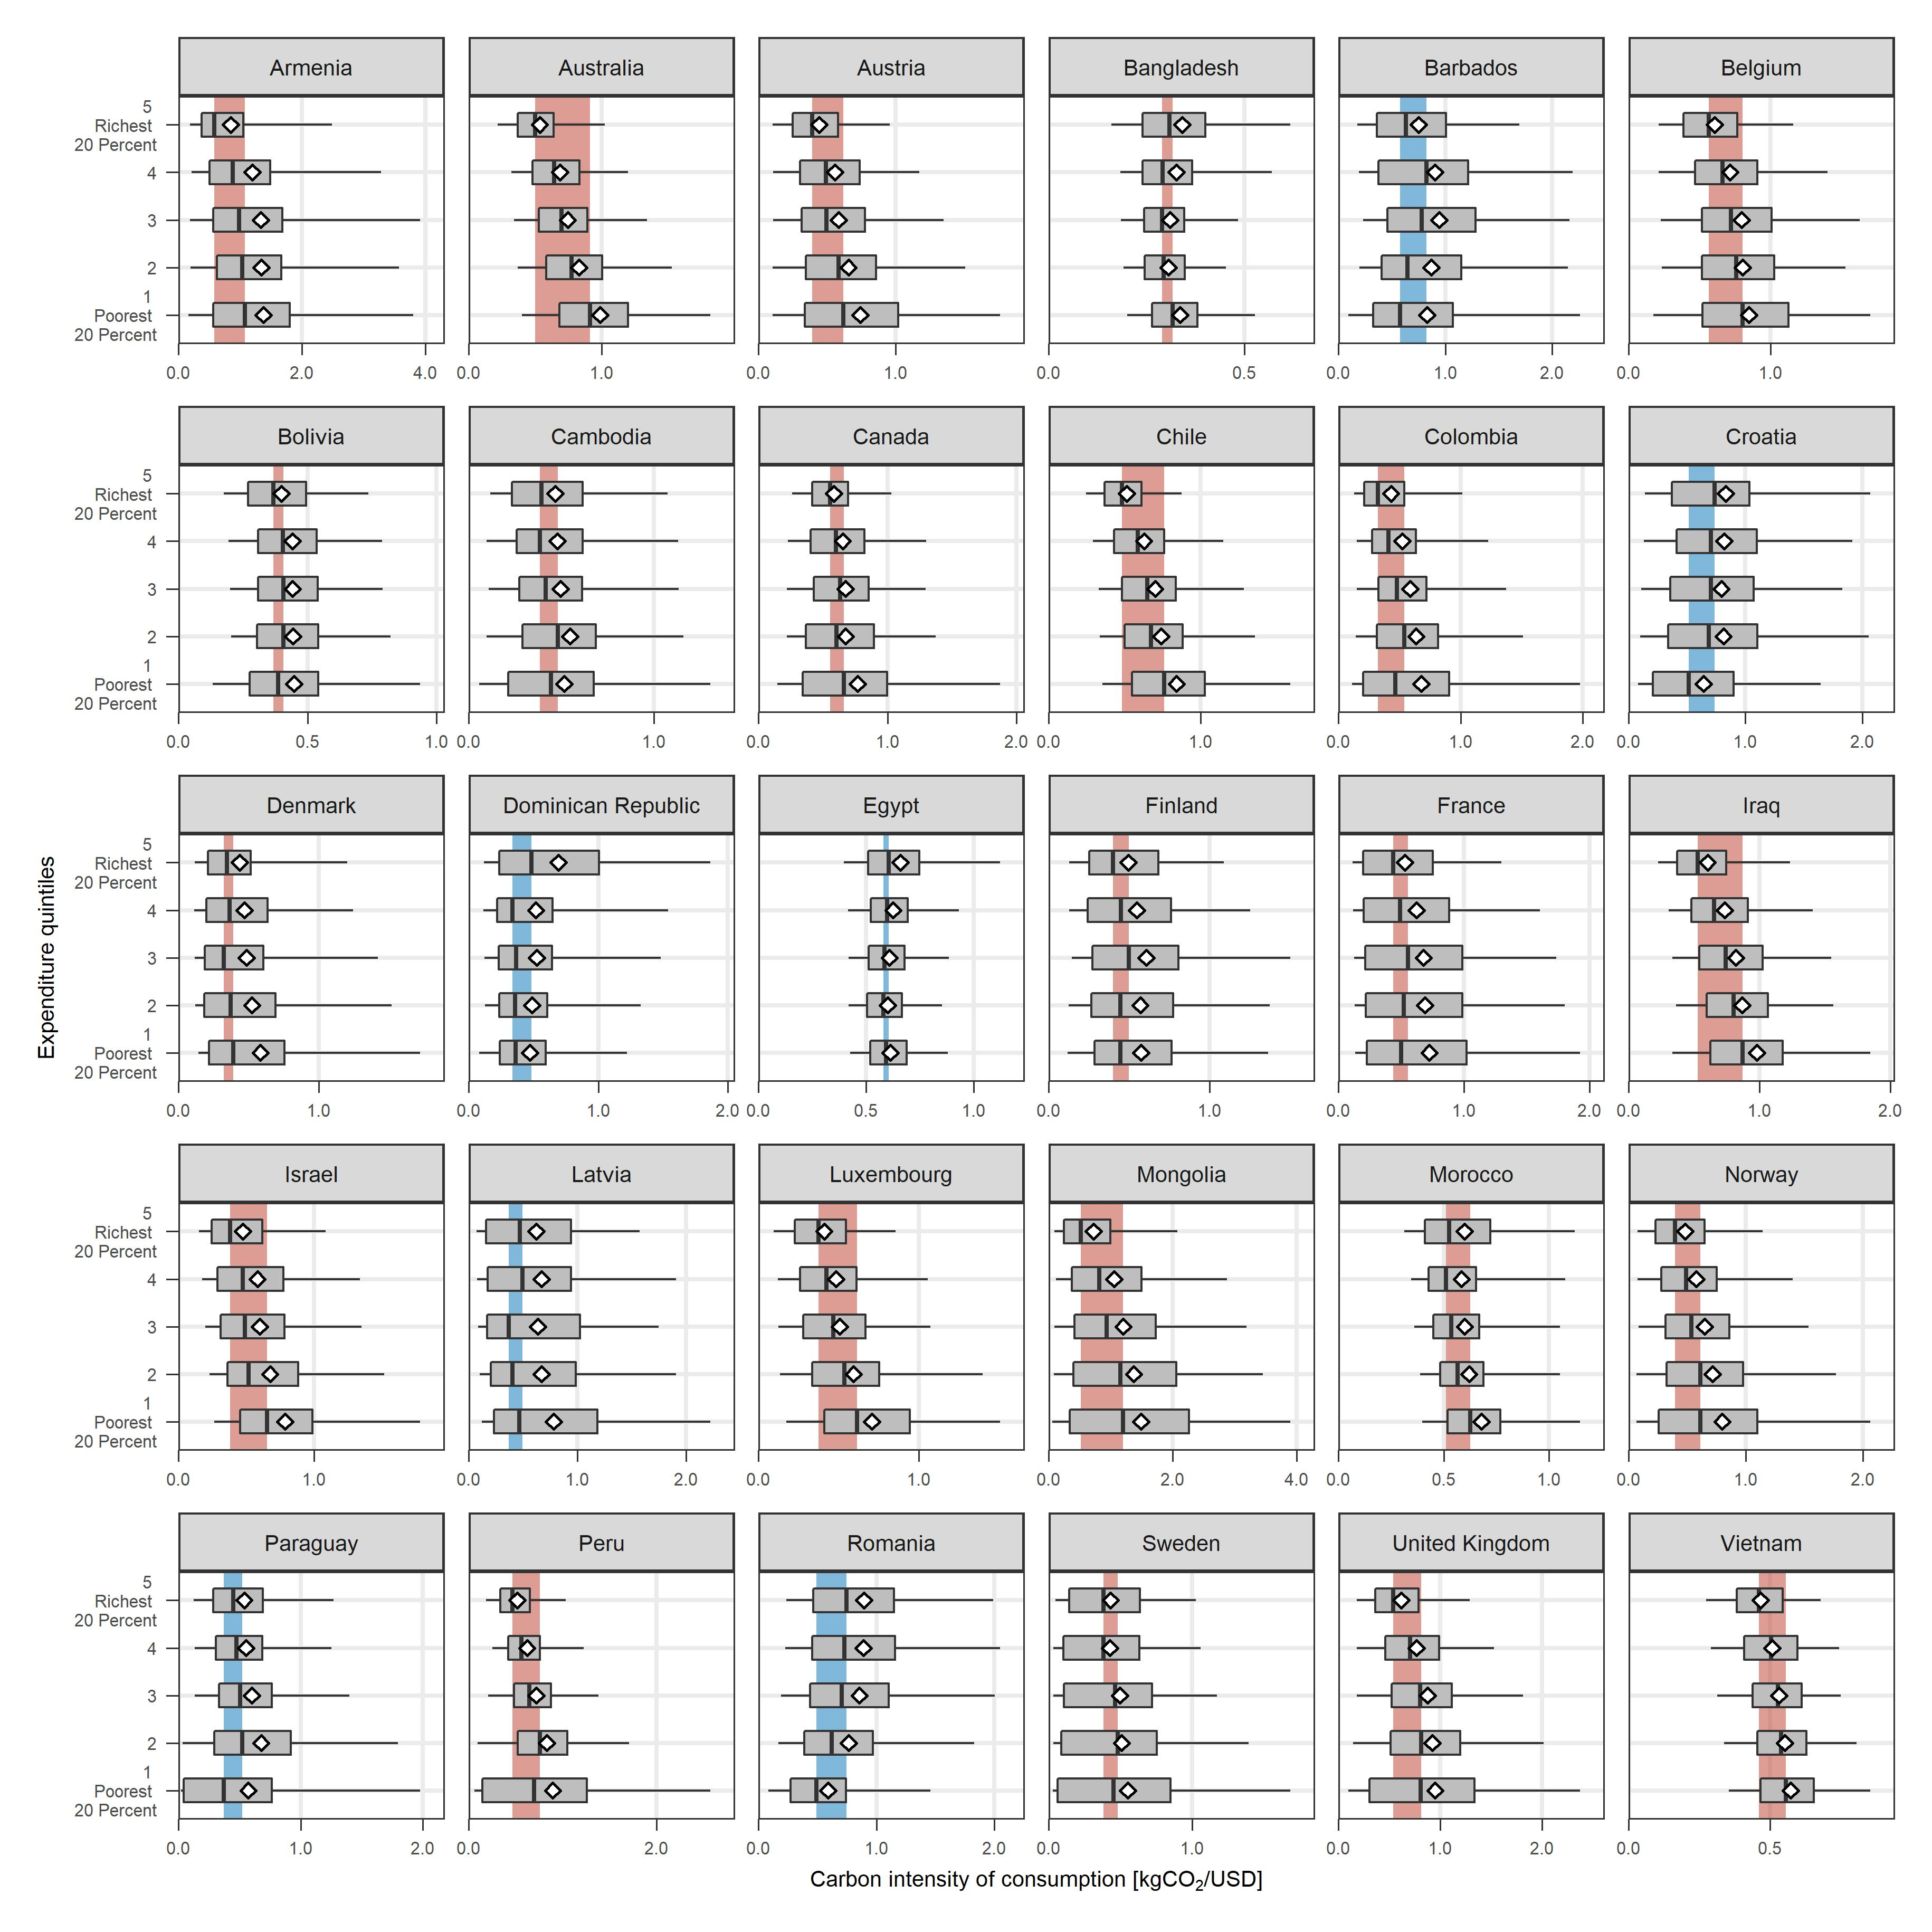
\includegraphics{1_Figures/Figures_Appendix/Figure_1_2017_Appendix_2.jpg}
  \begin{subcaption2}
    This figure displays the distribution of carbon intensity of consumption in kgCO$_{2}$/USD (x-axis) over expenditure quintiles (y-axis) for 30 countries. The first expenditure quintile comprises those 20\% of all households with least total expenditures per capita. The fifth expenditure quintile comprises those 20\% of all households with largest expenditures per capita. Within quintiles, boxes display the 25\textsuperscript{th} and the 75\textsuperscript{th} percentile; whiskers display the 5\textsuperscript{th} and 95\textsuperscript{th} percentile; rhombuses indicate the within-quintile average. Vertical coloured bands indicate the difference between the highest and the lowest quintile-level median carbon intensity of consumption. Blue bands indicate higher carbon intensities among richer households; red bands indicate higher carbon intensities among poorer households. See also Tables \ref{tab:A3} and \ref{tab:A7}.
  \end{subcaption2}
\end{subfigure}
\end{figure}

\clearpage

\begin{figure}[ht!]\ContinuedFloat
   \begin{subfigure}[b]{\textwidth}
  \centering
    \caption{Distribution of carbon intensities over expenditure quintiles - Part C} \label{fig:Quint_C}
  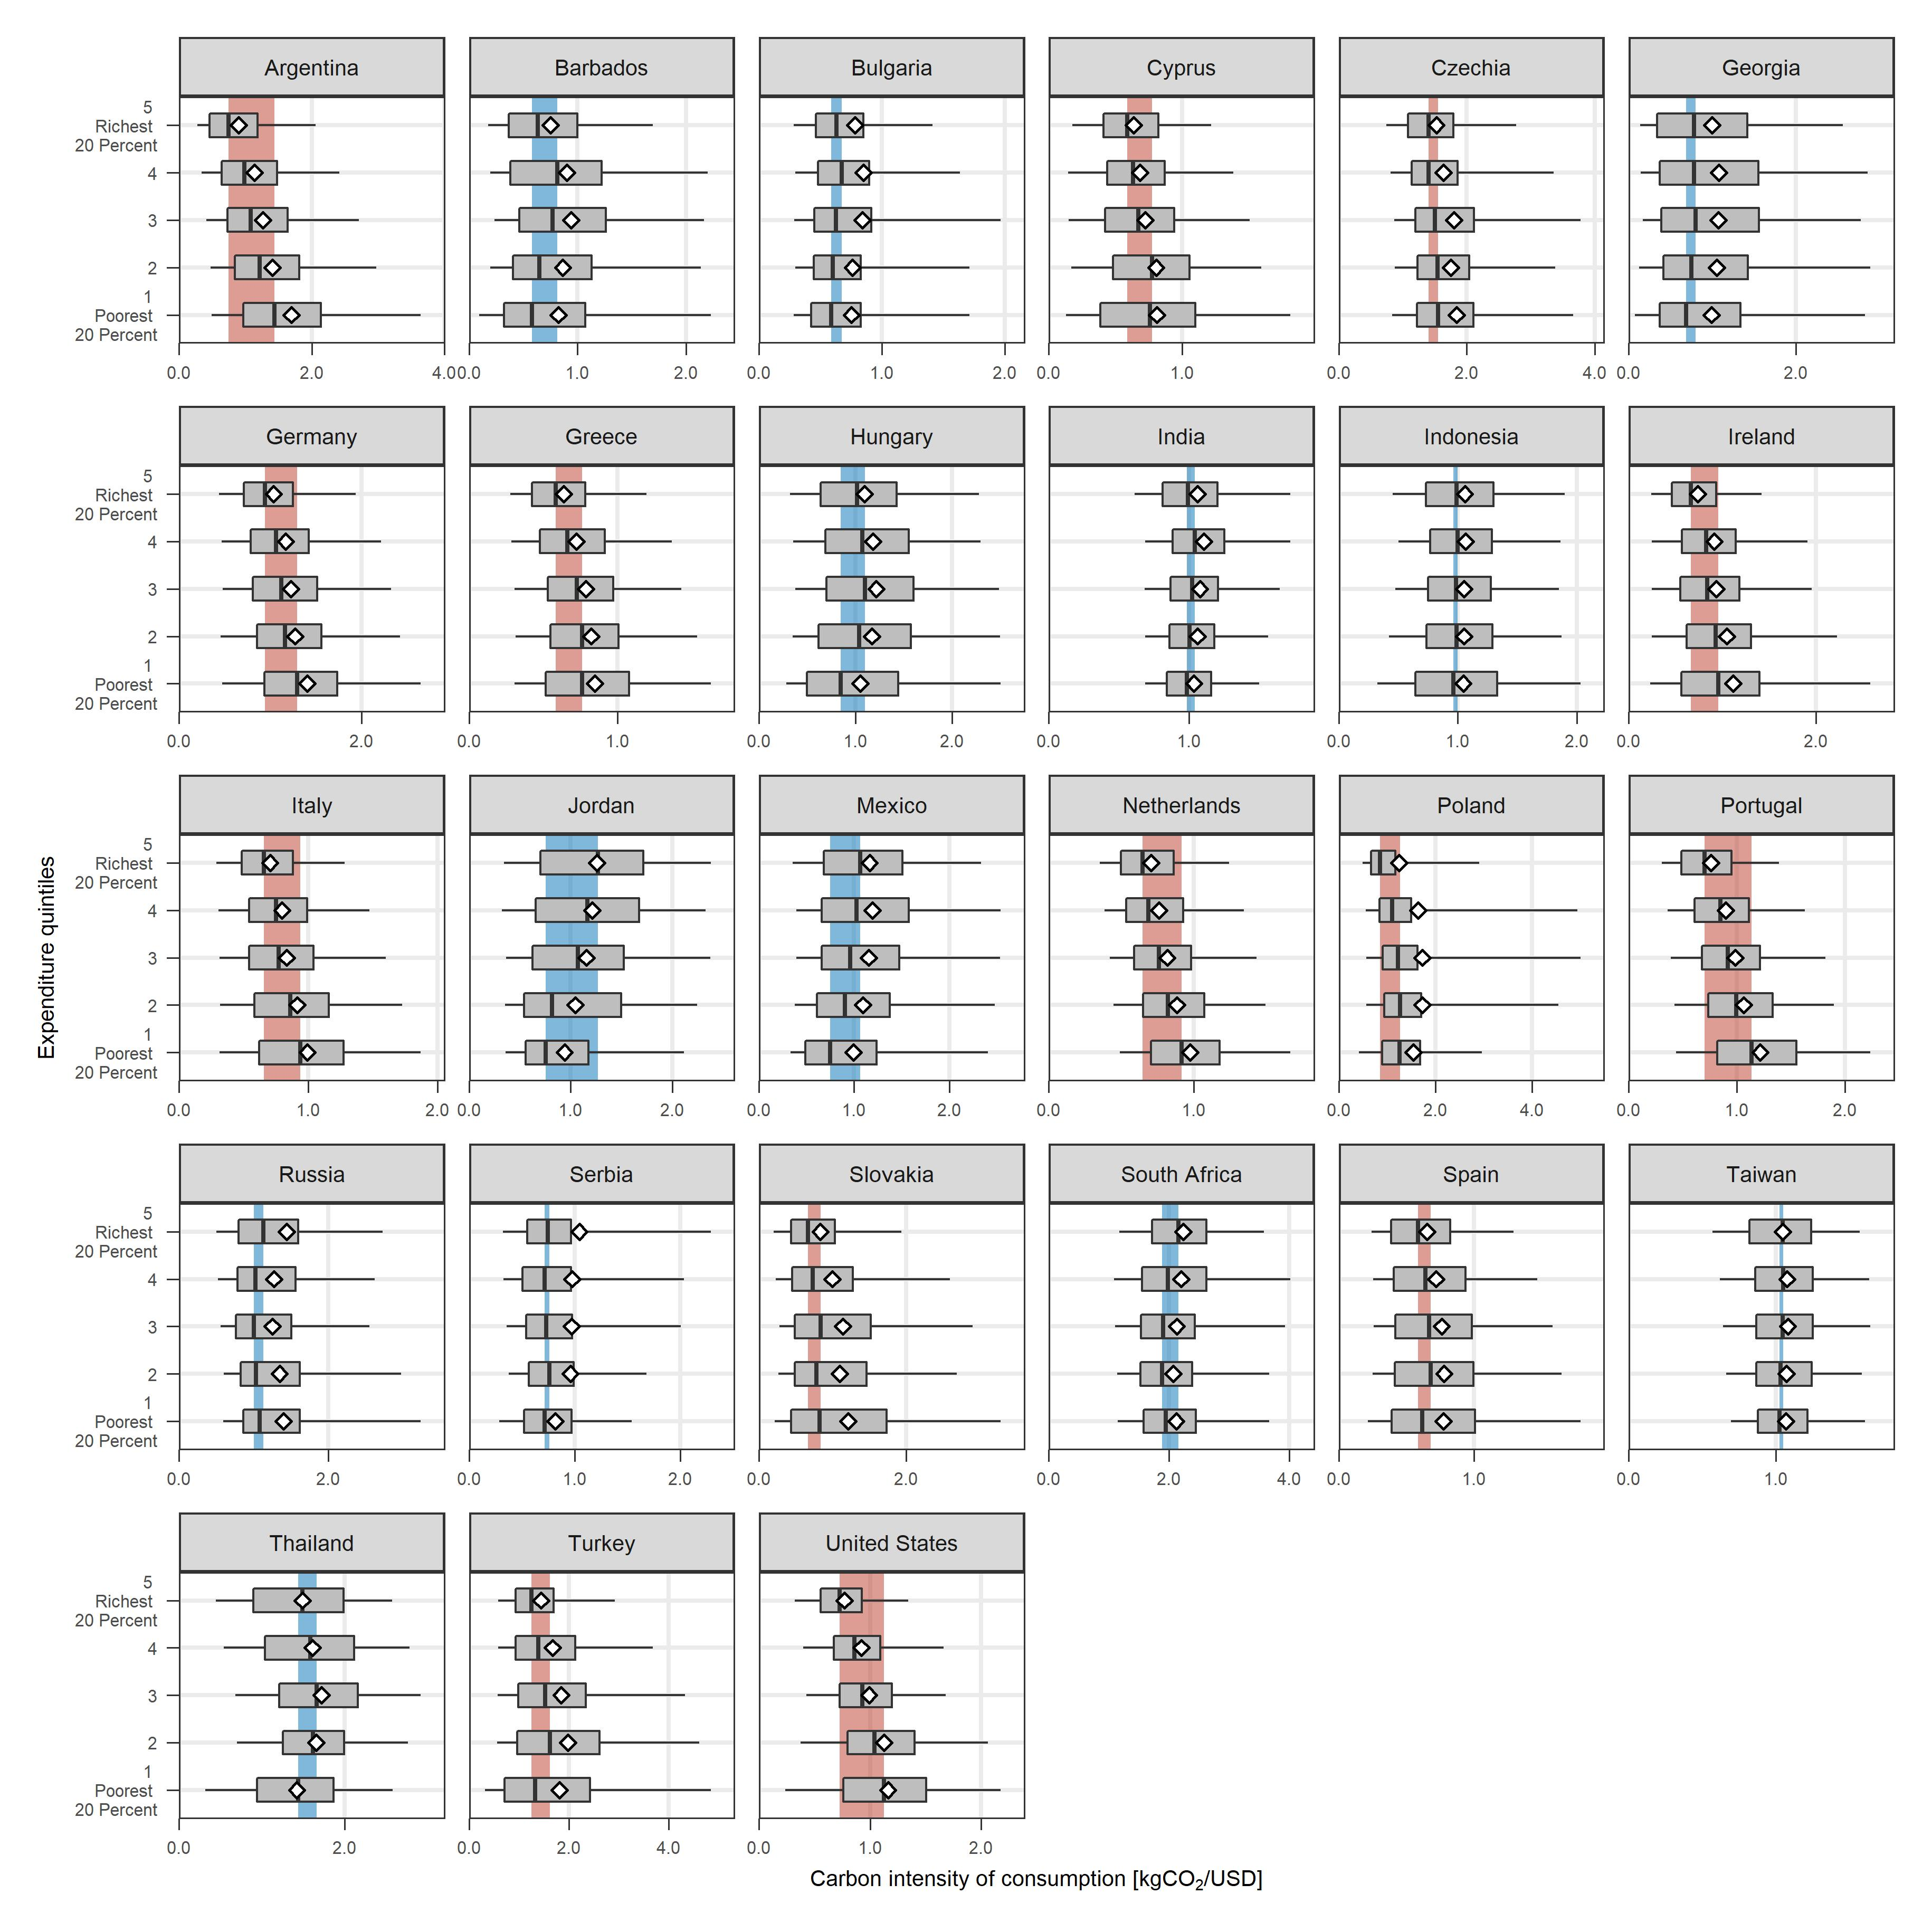
\includegraphics{1_Figures/Figures_Appendix/Figure_1_2017_Appendix_3.jpg}
  \begin{subcaption2}
    This figure displays the distribution of carbon intensity of consumption in kgCO$_{2}$/USD (x-axis) over expenditure quintiles (y-axis) for 27 countries. The first expenditure quintile comprises those 20\% of all households with least total expenditures per capita. The fifth expenditure quintile comprises those 20\% of all households with largest expenditures per capita. Within quintiles, boxes display the 25\textsuperscript{th} and the 75\textsuperscript{th} percentile; whiskers display the 5\textsuperscript{th} and 95\textsuperscript{th} percentile; rhombuses indicate the within-quintile average. Vertical coloured bands indicate the difference between the highest and the lowest quintile-level median carbon intensity of consumption. Blue bands indicate higher carbon intensities among richer households; red bands indicate higher carbon intensities among poorer households. See also Tables \ref{tab:A3} and \ref{tab:A7}.
  \end{subcaption2}
\end{subfigure}
\end{figure}